\documentclass[conference]{IEEEtran}
\usepackage{cite}
\usepackage{amsmath,amssymb,amsfonts}
\usepackage{algorithmic}
\usepackage{textcomp}
\usepackage{xcolor}
\usepackage{float}
\usepackage[T1]{fontenc}
\usepackage{graphicx}
\usepackage[utf8]{inputenc}
\usepackage[backend=biber, sorting=none]{biblatex}
\addbibresource{bibliography-biblatex.bib}
\usepackage[paperheight=27.94cm,paperwidth=21.59cm,left=2.54cm,right=2.54cm,top=2.54cm,bottom=2.54cm]{geometry}

\setlength\parindent{0pt}
\renewcommand{\arraystretch}{1.3}

\title{Sudoku Solver}
\begin{document}

\author{\IEEEauthorblockN{ Exdol Davy}
\IEEEauthorblockA{\textit{Undergraduate, Dept. Comp Sci.} \\
\textit{University of Central Florida}\\
Orlando, FL, USA \\
exdoldavy@knights.ucf.edu}
\and
\IEEEauthorblockN{ Douglas Glover}
\IEEEauthorblockA{\textit{Undergraduate, Dept. Comp Sci.} \\
\textit{University of Central Florida}\\
Orlando, FL, USA \\
DouglasGlover3@gmail.com}
\and
\IEEEauthorblockN{ Kashyap Rana}
\IEEEauthorblockA{\textit{Undergraduate, Dept. Comp Sci.} \\
\textit{University of Central Florida}\\
Orlando, FL, USA \\
kashyaprana202@gmail.com}
\and
\IEEEauthorblockN{ Matthew Singh}
\IEEEauthorblockA{\textit{Undergraduate, Dept. Comp Sci.} \\
\textit{University of Central Florida}\\
Orlando, FL, USA \\
matt18361@gmail.com}
\and
\IEEEauthorblockN{ Miguel Venero}
\IEEEauthorblockA{\textit{Undergraduate, Dept. Comp Sci.} \\
\textit{University of Central Florida}\\
Orlando, FL, USA \\
veneromiguel337@gmail.com}
}
\maketitle

\vspace{2\baselineskip}


\vspace{1\baselineskip}

\begin{abstract}
Malformed Sudoku puzzles (or Sudoku puzzles that have more than one solution) are an unlikely occurrence in today's world of computers, as opposed to when sudoku puzzles were created only by man. However, they are not impossible to be produced accidentally (or even on purpose). It has been mathematically proven by Gary McGuire, Bastian Tugemann, and Gilles Civario in 2012 [1] that a sudoku puzzle must provide at least 17 valid clues to contain exactly 1 unique solution. This project will provide further analysis upon this proof, while determining whether a sudoku puzzle can be solved or not.
\end{abstract}

\vspace{1\baselineskip}

\section{Introduction}
Sudoku is a Japanese puzzle game that requires players to fill all of 81 boxes presented in a 9 by 9 grid. The content of each box must be any integer between the interval of 1 through 9 inclusively. The 9 by 9 grid is also divided into 9 blocks (with 3 blocks being in each row and 3 blocks being in each column), each of which contain 9 boxes, therefore also being a 3 by 3 grid. The image below is an example of the 9 by 9 grid, with all 9 of the 3 by 3 gridded blocks.

\vspace{1\baselineskip}
\begin{figure}[H]
\centering
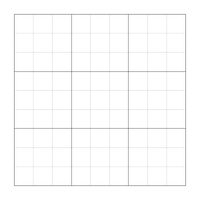
\includegraphics[width=5.11cm,height=4.87cm]{sudokujpg.jpg}
\end{figure}

\vspace{1\baselineskip}
Each sudoku puzzle typically starts off with at least 17 clues to be guaranteed to have a valid solution, but can contain more depending on the difficulty level. However, to successfully complete the game, the player must fill all empty boxes, in the 9 by 9 grid, such that each of the 9 blocks contain exactly 9 integers from the interval of 1 through 9 inclusive without repetition (each integer being within its own respective box). In addition to this, the boxes within each column and each row of the 9 by 9 grid must contain an integer from the interval of 1 through 9 inclusive without any duplicates being in each column and row respectively. 

\vspace{1\baselineskip}

\section{Methodology}
To better understand how to systematically solve a sudoku, we first created a single thread implementation of solving sudoku
which was a brute force method where it checks all possible values for each cell and iterates until the grid has been solved.
\\*

The next step was to come up with a multithreading approach for the problem. At first we thought to have two threads, one for the
column and one for the row, then both would work together to find all possible options for each cell to solve the sudoku.
This method does not properly use multithreading concepts to their full potential as it takes the single thread approach and assigns
threads to specific assignments. We decided that we did not want our project to move in this direction so we halted the
implementation of this approach.
\\*

After some discussions on what multithreading approaches we should take, more research was conducted.
To properly solve a grid we dived into understanding how average humans go about solving the sudoku, the pencil and paper algorithm.
A human uses the clues provided by the given numbers in the grid and uses logic to determine which values must
exist in particular cells. One of the most common strategies is to use the process of elimination, finding all the values that
are impossible in a cell. If there is only one value that remains possible, we know that it is the correct value.
\\*

The best way to combine common sudoku-solving strategies with multithreading was to first split the grid into pieces.
Assume we are working with a classic 9x9 sudoku grid. Each thread is to be given a row, column, and box (3x3 cell group).
This will split the grid evenly across nine separate threads. Each thread shares access to a three-dimensional matrix of boolean values
(9x9x9). The first two dimensions refer to a specific cell’s location in the grid, and the last dimension is used to track
which of the possible numbers for that cell have been eliminated.
\\*

This allows threads to share information on the values deemed impossible for each cell.
If all possible values in a cell are eliminated except for one, then the thread will mark it as the correct value for that cell.
\\*

There are four strategies that the program uses to determine the solution:
\vspace{1\baselineskip}
\begin{itemize}
    \item{If a number has been used in a row, column, or box, 
    then that number should be marked as impossible for all other cells in that row, column, or box.}

    \item{If a cell has all numbers deemed impossible except for one, 
    then that last number is the correct value for the cell.}

    \item{If a cell is the only cell in a row, column, or box where a number is possible, 
    then that number is the correct number for the cell.}

    \item{If there exists some number that must exist in both a specific row and box or a specific column and box, 
    then that number should be marked as impossible for any cells in the box outside the specific row or column.}
\end{itemize}
Using these four strategies allows the puzzle to be solved in a step-by-step method similar to how a person might solve it.


\section*{References}

\vspace{1\baselineskip}
[1] McGuire, Gary, et al. “There Is No 16-Clue Sudoku: Solving the Sudoku Minimum Number of Clues Problem.” NASA/ADS, https://ui.adsabs.harvard.edu/abs/2012arXiv1201.0749M/abstract. 


\printbibliography


\end{document}